\documentclass[a4paper,12pt]{article}
\usepackage[utf8x]{inputenc}
\usepackage[swedish]{babel}
\usepackage[T1]{fontenc}
\usepackage{graphicx}
\usepackage{placeins}
\usepackage{amsfonts, amsmath, amssymb}
\usepackage{ccfonts,euler}
\usepackage{wrapfig}
\usepackage{multirow}
\usepackage{caption}
\usepackage{enumerate}
\usepackage{comment}
\usepackage[includeheadfoot,margin=1.1in]{geometry}

\usepackage{listings}
\usepackage{color}

\definecolor{dkgreen}{rgb}{0,0.6,0}
\definecolor{gray}{rgb}{0.5,0.5,0.5}
\definecolor{mauve}{rgb}{0.58,0,0.82}

\lstset{frame=tb,
  language=Python,
  aboveskip=3mm,
  belowskip=3mm,
  showstringspaces=false,
  columns=flexible,
  basicstyle={\small\ttfamily},
  numbers=none,
  numberstyle=\tiny\color{gray},
  keywordstyle=\color{blue},
  commentstyle=\color{dkgreen},
  stringstyle=\color{mauve},
  escapeinside={\%*}{*)},
  breaklines=true,
  breakatwhitespace=true,
  tabsize=3,
  literate={å}{{\r a}}1 {ö}{{\"o}}1 {ä}{{\"a}}1 {Å}{{\r A}}1 {Ö}{{\"O}}1 {Ä}{{\"A}}1
}

\oddsidemargin -15mm
\evensidemargin -15mm
\marginparwidth 5mm
\topmargin -28mm
\textheight 282mm
\textwidth 190mm
\headheight 4mm
\headsep 4mm

\sloppy

\newcounter{iii}\setcounter{iii}{0}
\def\i{\bigskip\noindent\refstepcounter{iii}\textbf{\arabic{iii}.} }
%\def\iotst#1{\par \smallskip \mbox{}\refstepcounter{iii}\hspace*{#1}\textbf{\arabic{iii}.}}
\newcounter{pun}[iii]
\def\pu{\refstepcounter{pun}{\bf(\alph{pun})}\ }
\def\Pu{\par\noindent\mbox{}\refstepcounter{pun}{\phantom{\textbf{\arabic{iii}.}}\hspace{0.2mm}\bf(\alph{pun})}\ }

\def\ext{\subsection*{Extrauppgifter}}

\title{Programmering, Pepper - Pass 2}
\date{29 juli}

\makeatletter
\let\newtitle\@title
\let\newdate\@date
\makeatother
\begin{document}

  \renewcommand*\rmdefault{ppl}\normalfont\upshape
\pagestyle{empty}
\large
\section*{\newdate\ \  \newtitle}

\i

Fortsätt på klassen med komplexa tal och skapa metoder så att man kan addera, multiplicera, subtrahera, skriva ut talen, hämta ut real-/imaginärdel, hämta talet på rektangulär och polär form, jämföra olika tal mm. Kolla så funktionerna även fungerar med vanliga pythontal (typ att addera med x = 8.6).


Tips på funktioner att använda: \_\_add\_\_, \_\_mul\_\_ , \_\_sub\_\_ , \_\_div\_\_,  \_\_abs\_\_ , \_\_str\_\_, \_\_eq\_\_, \_\_ge\_\_, \_\_lt\_\_ .... 


Skapa en klass ''reell'' som ärver av komplexa tal och sätter imaginärdelen till 0. Den ska kunna användas både med andra reella tal, men också objekt av typen komplex och av vanliga pythontal (typ x = 8.3). Adderar man med ett komplex tal blir svaret naturligtvis komplext och inte reellt. 

Vill du kan du skapa barn till reell också som bara hantererar rationella tal, då får du spara täljaren och nämnaren som varsitt heltal för att undvika avrundningsfel i python. Se till att den klassen fungerar korrekt tillsammans med sina föräldrar (reell och komplex). 

\i

Labyrintkoden som vi nyss har gått igenom är rätt enkel att skriva, och löser oftast uppgiften inom rimlig tid. Men det finns specialfall som gör att DFS kommer ta rätt lång tid. Som tur är finns det en lösning på problemet som snabbar upp koden med nästan en faktor 100! Dynamisk programmering! Det handlar om att hela tiden spara den bästa lösningen som nått fram till ett speciellt tillstånd i spelet. Ibland kan det vara svårt att veta hur man ska spara en lösning i ett visst tillstånd, men just i labyrinten är det enkelt. Det är bara att spara minsta antalet drag för att nå fram till en viss ruta, i rutan själv. 

Modifiera er DFS lösning så att den sparar sina tillstånd i labyrinten. Dvs. ändra på besokt-arrayen från en boolsk array till en array med heltal. Uppdatera överallt där du använder dig av besokt variabeln. 

Koden borde bli mycket snabbare om ni gjort rätt. 


\i 
\begin{figure}[!ht]
\centering
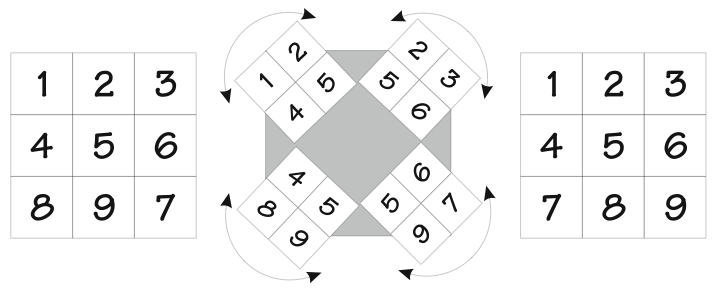
\includegraphics[width=0.7\textwidth]{Nokiaspel.png}
\caption{Till vänster ser vi en av många startmöjligheter. I mitten visas hur de fyra $2\times2$-kvadraterna kan roteras. Till höger visas målet.}
\label{fig:nokia}
\end{figure}

I flera av Nokias mobiltelefoner finns detta förströelsespel eller pussel. Pusslet går ut på att från ett givet utgångsläge, som till exempel till vänster i figur~\ref{fig:nokia}, nå fram till ordning och reda som till höger. I varje ställning finns åtta möjliga drag. Varje liten $2\times2$-kvadrat kan vridas $90^\circ$ medurs eller moturs i taget. Om man skulle göra fyra drag i följd med samma kvadrat i samma riktning skulle man vara tillbaka vid utgångsställningen.

Vi har undersökt att det aldrig behövs fler än 11 drag för att nå målet från vilken utgångsställning som helst. Din uppgift är att skriva ett program som tar emot en ställning och som bestämmer hur många drag den minst kräver för att nå målet. Ställningen (avläst rad för rad) ges till programmet som en sträng innehållande varje siffra i intervallet 1...9 exakt en gång.

\textbf{Körningsexempel:}

\begin{lstlisting}
Ställning ? 123456897
Denna ställning kräver 6 drag
\end{lstlisting}

\begin{comment}
def medurs(lista, x,y):
    lista = list(lista)
    tmp = lista[3*x+y]
    lista[3*x+y] = lista[3*x+y+1]
    lista[3*x+y+1] = lista[3*(x+1)+y+1]
    lista[3*(x+1)+y+1] = lista[3*(x+1)+y]
    lista[3*(x+1)+y] = tmp
    return tuple(lista)

def moturs(lista, x,y):
    lista = list(lista)
    tmp = lista[3*x+y]
    lista[3*x+y] = lista[3*(x+1)+y]
    lista[3*(x+1)+y] = lista[3*(x+1)+y+1]
    lista[3*(x+1)+y+1] = lista[3*x+y+1]
    lista[3*x+y+1] = tmp
    return tuple(lista)

vis = set()

def solve(lista):

    que = [lista]
    i = 0
    while que:
        que2 = []

        for state in que:

            if state == (1,2,3,4,5,6,7,8,9):
                print("Answer: ", i)
                return i

            for x in range(2):
                for y in range(2):
                    nextState = medurs(state,x,y)

                    if nextState not in vis:
                        vis.add(nextState)
                        que2.append(nextState)

                    nextState = moturs(state,x,y)
                    if nextState not in vis:
                        vis.add(nextState)
                        que2.append(nextState)
        i += 1
        que = que2
    return 1000000000000000
solve((1,2,3,4,5,6,8,9,7))
\end{comment}


\i

Senet är ett uråldrigt egyptiskt brädspel som hittats i otaliga gravar. Reglerna är okända men en av de vanligaste rekonstruktionerna beskrivs här. Spelplanen kan betraktas som en serie med rutor där vi i denna uppgift endast bryr oss om de första 15. De två spelarna, som vi kallar A och B, har vardera 5 pjäser som vid spelets början alltid står uppställda enligt översta schemat i figur~\ref{fig:senet}. Spelarna turas om att göra drag, A har första draget. I varje drag kastar spelaren några stickor, vilka tillsammans utgör en slags tärning som kan anta värdena 1, 2, 3, 4 eller 5. Därefter väljer spelaren en av sina pjäser och flyttar den framåt med så många steg som tärningen visade. För att vara ett godkänt drag måste pjäsen sluta på en ruta som antingen är tom eller innehåller en obevakad motståndarpjäs. I det senare fallet flyttas motståndarpjäsen tillbaka till den ruta varifrån den flyttade pjäsen kom, så att pjäserna i praktiken byter plats. En pjäs är obevakad om det inte finns en likadan pjäs i någon av de två angränsande rutorna.


\begin{figure}[!ht]
\centering
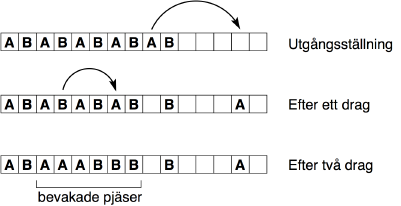
\includegraphics[width=0.5\textwidth]{Senet.png}
\caption{Utgångsställningen samt ställningarna efter dragen i exemplet nedan.}
\label{fig:senet}
\end{figure}

Du ska skriva ett program som givet pjäsernas nuvarande positioner bestämmer det minimala antalet drag N som har spelats, samt en möjlig sådan dragsekvens.

Programmet ska fråga efter en sträng med längd 15, där varje tecken beskriver en ruta på spelplanen: A för en pjäs tillhörande spelare A, B för en pjäs tillhörande spelare B och . (punkt) för en tom ruta. Det finns alltid fem A:n, fem B:n och fem punkter i strängen.

Programmet ska skriva ut den kortaste dragsekvensen som leder från utgångsställningen till den inmatade ställningen. Närmare bestämt ska programmet skriva ut en rad med N tal i intervallet 1..5, där varje tal anger hur många steg som har tagits i respektive drag (första talet indikerar första draget etc.). Vilken pjäs som flyttats i varje drag behöver inte anges. Om det finns flera sekvenser med minimal längd kan programmet ange vilken som helst av dem. I samtliga testfall är $N \le 6$. Notera att N kan vara udda, d.v.s. A kan ha gjort ett drag mer än B.

\begin{comment}

def isInvalid(state, fromPos, toPos, A_turn):
    if A_turn and state[fromPos] != 'A':
        return True
    if not A_turn and state[fromPos] != 'B':
        return True
    if toPos < 14 and state[toPos] == state[toPos+1] and state[toPos] != '.':
        return True
    if toPos > 0 and state[toPos-1] == state[toPos] and state[toPos] != '.':
        return True
    return False

startState = tuple(list('ABABABABAB.....'))
vis = set(startState)

def solve(endState):

    que = [(startState, ())]
    i = 0
    while que:
        que2 = []

        for (state, dragsekvens) in que:

            if state == endState:
                return dragsekvens

            for fromPos in range(15):
                for toPos in range(15):
                    if abs(fromPos - toPos) > 5:
                        continue

                    if isInvalid(state, fromPos, toPos, i%2+1):
                        continue

                    nextState = list(state)
                    nextState[fromPos], nextState[toPos] = nextState[toPos], nextState[fromPos]
                    nextState = tuple(nextState)
                    if nextState in vis:
                        continue
                    vis.add(nextState)
                    que2.append((nextState, dragsekvens + state + ('\n',)))
        i += 1
        que = que2
    return 1000000000000000

endState = "ABAAABBB.B...A."
A = solve(tuple(list(endState)))
for i in A:
    print(i, end='')
print(endState)
\end{comment}

\textbf{Körningsexempel:}

\begin{lstlisting}
Ställning ? ABAAABBB.B...A. 
Dragsekvens: 5 3 
\end{lstlisting}

\i


\begin{figure}[!ht]
\centering
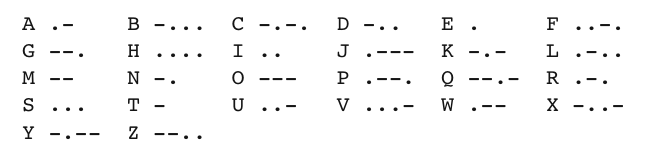
\includegraphics[width=0.7\textwidth]{Morse.png}
\caption{Tabell över morsekoderna}
\label{fig:morse}
\end{figure}


Tabellen ovan visar Morsealfabetet. Punkter och streck används för att beteckna korta respektive långa signaler. Normalt lämnas morsemeddelanden med ett uppehåll mellan varje bokstav, till exempel --. . - som står för ordet GET. Men av en obestämd anledning kommer det just nu in meddelanden i en oavbruten följd av långa och korta signaler, alltså utan uppehåll mellan bokstäverna. GET-signalen blir då --..- och kan därför stå för många andra bokstavssekvenser, t.ex. MU. Skriv ett program som tar emot en följd av streck och punkter, och som sedan skriver ut varje möjlig kombination av bokstäver som svarar mot den givna indatasträngen.


\textbf{Indata}
På första raden står signalsträngen, som består av högst 15 tecken. 

\textbf{Utdata}
Programmet ska skriva ut alla möjliga bokstavssekvenser som svarar mot den givna indatasträngen. Sekvenserna ska skrivas ut i alfabetisk ordning med en per rad. Endast versalerna A-Z får förekomma.



\textbf{Körningsexempel:}
\begin{lstlisting}
Morsekod? --..- 
Möjliga sekvenser: 
GA, GET, MEA, MEET, MIT, MU, TDT, TNA, TNET, TTEA, TTEET, TTIT, TTU, TX, ZT, 
Morsekod? ..-
EA, EET, IT, U, 
\end{lstlisting}

\begin{comment}
# MÅSTE HA PYTHON 3.6 eller högre för att få dem i bokstavsordning
morsekod = {".-": "A", "-...": "B", "-.-.": "C", "-..": "D", ".": "E", "..-.": "F", "--.": "G", "....": "H", "..": "I", ".---": "J", "-.-": "K", ".-..": "L", "--": "M", "-.": "N", "---": "O", ".--.": "P", "--.-": "Q", ".-.": "R", "...": "S", "-": "T", "..-": "U", "...-": "V", ".--": "W", "-..-": "X", "-.--": "Y", "--..": "Z"}

text = input("Morsekod? ")

def rekurs(kvar, komb):
    if not kvar:
        print(komb)
        return
    for morse, letter in morsekod.items():
        if kvar.startswith(morse):
            rekurs(kvar[len(morse):], komb + letter)
                
rekurs(text, "")
\end{comment}

\pagebreak

\i


\begin{figure}[!ht]
\centering
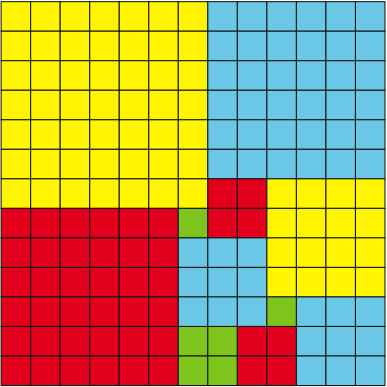
\includegraphics[width=0.2\textwidth]{kvadrater.png}
\caption{}
\label{fig:kvadrater}
\end{figure}


I figur~\ref{fig:kvadrater} ser du en kvadrat ($13\times13$) som består av 11 mindre kvadrater, som också är det minsta antal ''småkvadrater'' som krävs för att skapa en kvadrat av denna storlek.

Skriv ett program som tar emot den stora kvadratens sida S , där $2 \le S \le 17$, och bestämmer det minsta antal mindre kvadrater som behövs för att lägga pusslet.

\textbf{Körningsexempel:}
\begin{lstlisting}
Kvadratens sida ? 13 
Det behövs minst 11 kvadrater
\end{lstlisting}
\begin{comment}
# Kvadratens bredd och höjd.
N = int(input("Kvadratens sida? "))

#Minsta antalet drag som krävs är åtminstone inte
#fler än 2N, vilket är en enkel lösning där man
#bara placerat ut en stor fet kvadrat och övriga
#mindre kvadrater av storlek 1.
minsta = 2*N+1

# Vår kvadrat som vi ska fylla.
kvadrat = [[False for i in range(N)] for j in range(N)]


def findFirstEmpty():
    """ Metod som letar rätt på en ledig ruta och retunerar dess koordinat i form av en punkt. """
    for i in range(N): # y-koordinat.
        for j in range(N): # x-koordinat.
            # Om rutan är ledig så retunerar vi den.
            if not kvadrat[i][j]:
                return (j,i)
    # Kvadraten är full.
    return ()



def isValid(p, size):
    """
    Retunerar huruvida det är tillåtet att lägga en kvadrat av storlek size
    med sitt övre vänstra hörn i punkten/rutan p. Dvs metoden kollar att
    kvadraten man tänker lägga inte överlappar andra eller går utanför.
    """
    # För stora kvadrater tycker ingen om.
    if p[0] + size > N or p[1] + size > N:
        return False
    # Går igenom det område som kvadraten kommer att täcka.
    for i in range(p[1], p[1]+size): # y-koordinat.
        for j in range(p[0], p[0]+size): # x-koordinat.
            # Om rutan redan var upptagen så är draget otillåtet.
            if kvadrat[i][j]:
                return False
    # Kvadraten har klarat testerna.
    return True



def putQuad(p, size):
    """ Lägger en kvadrat av storlek size på punkten/rutan p."""
    # Markerar de rutor som kvadraten ska täcka som upptagna.
    for i in range(p[1], p[1]+size):
        for j in range(p[0], p[0]+size):
            kvadrat[i][j] = True


def removeQuad(p, size):
    """ Tar bort en kvadrat av storlek size som börjar i punkten p."""
    for i in range(p[1], p[1]+size):
        for j in range(p[0], p[0]+size):
            kvadrat[i][j] = False


def rek(used):
    """ Vår rekursiva metod som testar att lägga ut kvadrater. 
    used: Hur många kvadrater vi använt. """
    global minsta
    # Om vi redan har en bättre lösning, dumt att fortsätta.
    if used >= minsta:
        return
    # Hittar första tomma rutan.
    p = findFirstEmpty()

    # Om svaret var null så betyder det att kvadraten är full
    # och vi har funnit den hittills bästa lösningen.
    if not p:
        minsta = used
    else: # Annars så fortsätter vi att testa lägga ut kvadrater på punkten p.
        # Vi börjar att testa med större kvadrater. (Det är smartare.)
        for size in range(N-1, 0, -1):
            # Om det är tillåtet att lägga kvadraten så gör vi det.
            if isValid(p, size):
                # Lägger kvadraten med storleken size på punkten p.
                putQuad(p, size)
                
                # Nu har vi använt en kvadrat och testar att lägga på en annan punkt.
                rek(used+1)
                
                # Tar bort kvadraten, är ju inte säkert att den är optimal.
                removeQuad(p, size)



# Om sidan är jämn så är lösningen trivial.
if N%2 == 0:
    minsta = 4
else: # Annars får vi testa oss fram.
    # Från början har vi lagt ut noll mindre kvadrater.
    rek(0)

#Skriver ut svaret.
print("Det behövs minst " + str(minsta) + " kvadrater")
\end{comment}


\i
På mitt jobb finns en colaautomat där en burk Coca-Cola kostar 8 kr. Maskinen har ett myntinkast som accepterar 1 kr, 5 kr och 10 kronorsmynt. Efter att tillräckligt många mynt har stoppats in kan jag trycka på Cola-knappen och få ut en Cola och eventuell växel. Växeln ges alltid tillbaka med det minsta antalet möjliga mynt. Denna procedur upprepas tills jag köpt så många Cola-burkar som jag vill ha. Jag kan bara köpa en burk åt gången. Om jag t.ex. skulle stoppa in 16 kr och trycka på Cola-knappen skulle jag få ut en burk och 8 kronor i växel (en 5-krona och 3 enkronor).

Givet hur många burkar jag vill köpa, samt hur många mynt jag har av varje valör, vad är det minsta antalet mynt jag behöver stoppa in i maskinen för att köpa så många burkar som jag vill ha? Jag kan ta upp mynt som kommer ut som växel. Du kan utgå ifrån att maskinen har obegränsat med mynt i växel.

Programmet ska, i tur och ordning, fråga efter hur många Cola-burkar jag vill köpa (mellan 1 och 40), antalet 1-kronors mynt jag har (mellan 0 och 100), antalet 5-kronors mynt (mellan 0 och 20), och antalet 10-kronors mynt (mellan 0 och 10). Programmet ska skriva ut det minsta antal mynt jag behöver stoppa i myntinkastet. Du kan utgå ifrån att jag har tillräckligt med pengar för att köpa alla Cola-burkar jag vill ha.


\textbf{Körningsexempel:}
\begin{lstlisting}
Antal burkar ? 2
Antal 1-kronor ? 2
Antal 5-kronor ? 1
Antal 10-kronor ? 1
Du behöver stoppa in 5 mynt.

Antal burkar ? 3
Antal 1-kronor ? 20
Antal 5-kronor ? 1
Antal 10-kronor ? 1
Du behöver stoppa in 12 mynt.
\end{lstlisting}

\begin{comment}
burkar = int(input("Antal burkar: "))
n1 = int(input("antal 1: "))
n5 = int(input("antal 5: "))
n10 = int(input("antal 10: "))

cache = dict()
ans = 1000000000000000000000
def solve(burkar, n1,n5,n10, cnt):
    global ans

    if burkar == 0:
        ans = min(ans, cnt)
        return 0
    if (burkar,n1,n5,n10) in cache:
        if cnt <= cache[(burkar,n1,n5,n10)]:
            return

    cache[(burkar,n1,n5,n10)] = cnt

    if n10 >= 1 and n1 >= 3: # Gor vaxlingshandling
        solve(burkar-1, n1-3, n5+1, n10-1, cnt+4)
    if n5 >= 1 and n1 >= 3:
        solve(burkar-1, n1-3, n5-1, n10, cnt+4)
    if n10 >= 1:
        solve(burkar-1, n1+2, n5, n10-1, cnt+1)
    if n5 >= 2:
        solve( burkar-1, n1+2, n5-2, n10, cnt+2)
    if n1 >= 8:
        solve(burkar-1, n1-8, n5, n10, cnt+8)

solve(burkar, n1,n5,n10,0)

print("Man måste använda: ", ans, " mynt")
\end{comment}

\end{document}